\documentclass{beamer}
\usepackage[utf8]{inputenc}

\usetheme{Madrid}
\usecolortheme{default}
\usepackage{amsmath,amssymb,amsfonts,amsthm}
\usepackage{txfonts}
\usepackage{tkz-euclide}
\usepackage{listings}
\usepackage{adjustbox}
\usepackage{array}
\usepackage{tabularx}
\usepackage{gvv}
\usepackage{lmodern}
\usepackage{circuitikz}
\usepackage{tikz}
\usepackage{graphicx}

\setbeamertemplate{page number in head/foot}[totalframenumber]

\usepackage{tcolorbox}
\tcbuselibrary{minted,breakable,xparse,skins}



\definecolor{bg}{gray}{0.95}
\DeclareTCBListing{mintedbox}{O{}m!O{}}{%
  breakable=true,
  listing engine=minted,
  listing only,
  minted language=#2,
  minted style=default,
  minted options={%
    linenos,
    gobble=0,
    breaklines=true,
    breakafter=,,
    fontsize=\small,
    numbersep=8pt,
    #1},
  boxsep=0pt,
  left skip=0pt,
  right skip=0pt,
  left=25pt,
  right=0pt,
  top=3pt,
  bottom=3pt,
  arc=5pt,
  leftrule=0pt,
  rightrule=0pt,
  bottomrule=2pt,
  toprule=2pt,
  colback=bg,
  colframe=orange!70,
  enhanced,
  overlay={%
    \begin{tcbclipinterior}
    \fill[orange!20!white] (frame.south west) rectangle ([xshift=20pt]frame.north west);
    \end{tcbclipinterior}},
  #3,
}
\lstset{
    language=C,
    basicstyle=\ttfamily\small,
    keywordstyle=\color{blue},
    stringstyle=\color{orange},
    commentstyle=\color{green!60!black},
    numbers=left,
    numberstyle=\tiny\color{gray},
    breaklines=true,
    showstringspaces=false,
}
%------------------------------------------------------------
%This block of code defines the information to appear in the
%Title page
\title %optional
{1.5.14}
\date{August 21,2025}
%\subtitle{A short story}

\author % (optional)
{Harsha-EE25BTECH11026}



\begin{document}


\frame{\titlepage}
\begin{frame}{Question}
Points P and Q trisect the line segment joining the points A $\brak{-2, 0}$ and B$\brak{0,8}$ such that P is nearer to A. Find the coordinates of points P and Q.
\end{frame}



\begin{frame}{Theoretical Solution}

Let the vectors $\vec{P}$ and $\vec{Q}$ be 
\begin{align}
    \vec{P}=\begin{myvec}{x_1\\y_1}\end{myvec} \;, \vec{Q}=\begin{myvec}{x_2\\y_2} \end{myvec}
\end{align}
Given the points,
\begin{align}
    \vec{A}=\begin{myvec}{-2\\0}\end{myvec}
    \vec{B}=\begin{myvec}{0\\8}\end{myvec}
\end{align}
we can use the internal division formula to find the points $\vec{P}$ and $\vec{Q}$.\\

\end{frame}

\begin{frame}{Equation}
\textbf{Internal division formula for a vector $\vec{R}$ which divides the line formed by vectors $\vec{A}$ and $\vec{B}$ in the ratio m:n is given by}
\begin{align}
    \vec{R}=\frac{m\vec{B}+n\vec{A}}{m+n}
\end{align}
\end{frame}
\begin{frame}{Theoretical Solution}
To find vector $\vec{P}$, as it is near the point A, it divides the line formed by line A and B in ratio 1:2.\\
Therefore,\\
\begin{align}
    \vec{P}=\frac{2\times\begin{myvec}{-2 \\ 0}\end{myvec}+1\times\begin{myvec}{0\\8}\end{myvec}}{1+2}
\end{align}
\begin{align}
    \vec{P}=\begin{myvec}{\frac{-4}{3}\\\frac{8}{3}}\end{myvec}
\end{align}
\end{frame}

\begin{frame}{Theoretical Solution}
To find vector $\vec{Q}$, as it is near the point B, it divides the line formed by line A and B in ratio 2:1.\\
Therefore,\\

\begin{align}
    \vec{Q}=\frac{1\times\begin{myvec}{-2 \\ 0}\end{myvec}+2\times\begin{myvec}{0\\8}\end{myvec}}{2+1}
\end{align}
\begin{align}
    \vec{Q}=\begin{myvec}{\frac{-2}{3}\\\frac{16}{3}}\end{myvec}
\end{align}
\end{frame}
\begin{frame}[fragile]
    \frametitle{C Code - Internal division formula}

    \begin{lstlisting}

\#include <stdio.h>

void find\_section\_point(double \;x1, double \;y1, double \;x2, double y2, double m, double n, double* x, double* y) {
    *x = (m * x2 + n * x1) / (m + n);
    *y = (m * y2 + n * y1) / (m + n);
    \end{lstlisting}
\end{frame}

\begin{frame}[fragile]
    \frametitle{Python Code}
    \begin{lstlisting}
import ctypes
import numpy as np
import matplotlib as mp
import matplotlib.pyplot as plt

lib = ctypes.CDLL('./libintdiv_formula.so')
lib.find_section_point.argtypes = [ctypes.c_double, ctypes.c_double, ctypes.c_double,
                                   ctypes.c_double, ctypes.c_double, ctypes.c_double,
                                   ctypes.POINTER(ctypes.c_double), ctypes.POINTER(ctypes.c_double)]
lib.find_section_point.restype = None


    \end{lstlisting}
\end{frame}

\begin{frame}[fragile]
    \frametitle{Python Code}
    \begin{lstlisting}
def find_section_point(x1, y1, x2, y2, m, n):
    x = ctypes.c_double()
    y = ctypes.c_double()
    lib.find_section_point(x1, y1, x2, y2, m, n, ctypes.byref(x), ctypes.byref(y))
    return (x.value, y.value)
    \end{lstlisting}
\end{frame}

\begin{frame}[fragile]
    \frametitle{Python Code}
    \begin{lstlisting}
# Given points
A = (-2,0)
B = (0,8)

# Find P such that AP:PB=1:2
P = find_section_point(A[0], A[1], B[0], B[1], 1, 2)
# Find Q such that AQ:QB=2:1
Q = find_section_point(A[0], A[1], B[0], B[1], 2, 1)

# Format results
P_formatted = (round(P[0], 2), round(P[1], 2))
Q_formatted = (round(Q[0], 2), round(Q[1], 2))

print(f"P: {P_formatted}")
print(f"Q: {Q_formatted}")
    \end{lstlisting}
\end{frame}

\begin{frame}[fragile]
    \frametitle{Python Code}
    \begin{lstlisting}
# Plotting
plt.figure(figsize=(8, 8))

# Line AB
plt.plot([A[0], B[0]], [A[1], B[1]], 'ro-', label='AB')

# Points P and Q
plt.plot(*P_formatted, 'go', label='P', markersize=8)   # green
plt.plot(*Q_formatted, 'bo', label='Q', markersize=8)   # blue

# Labels
plt.text(A[0]+0.1, A[1], 'A', fontsize=12, ha='right')
plt.text(B[0]+0.1, B[1], 'B', fontsize=12, ha='right')
plt.text(*P_formatted, f'P {P_formatted}', fontsize=12, ha='right', color='green')
plt.text(*Q_formatted, f'Q {Q_formatted}', fontsize=12, ha='left', color='blue')
    \end{lstlisting}
\end{frame}
\begin{frame}[fragile]
    \frametitle{Python Code}
    \begin{lstlisting}
mp.use("TkAgg")
plt.xlabel('x')
plt.ylabel('y')
plt.title('Trisection of line AB by points P and Q')
plt.legend()
plt.grid(True)
plt.gca().set_aspect('equal', adjustable='box')

# Save before show
plt.savefig("/home/user/Matrix/Matgeo_assignments/1.5.14/figs/Figure_1.png", dpi=300, bbox_inches='tight')
plt.show()
    \end{lstlisting}
\end{frame}


\begin{frame}{Plot}
    \centering
    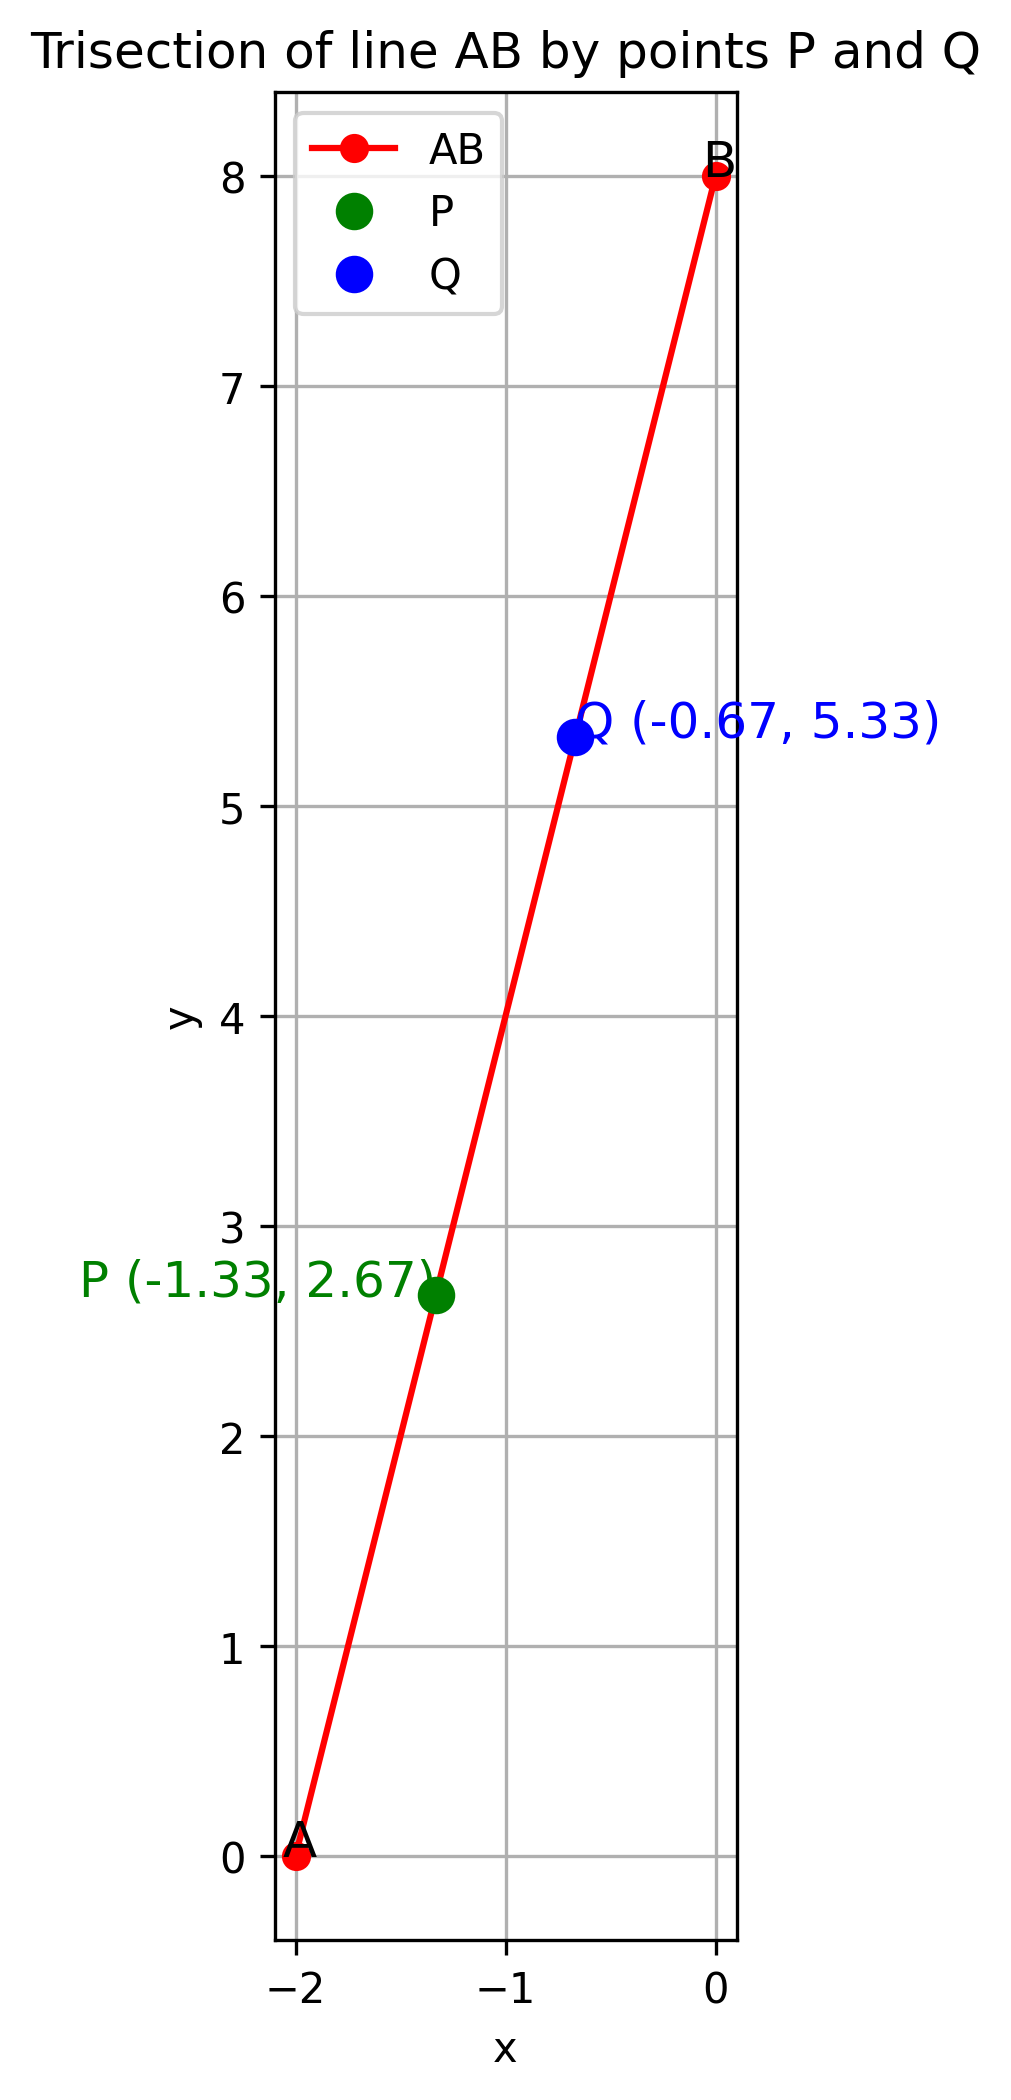
\includegraphics[width=\columnwidth, height=0.8\textheight, keepaspectratio]{figs/Figure_1.png}     
\end{frame}


\end{document}